% Options for packages loaded elsewhere
\PassOptionsToPackage{unicode}{hyperref}
\PassOptionsToPackage{hyphens}{url}
%
\documentclass[
]{article}
\title{Seoul Bike Data}
\author{William K Davis III \and Pei-Yin Yang \and Max Kutschinski}
\date{2022-06-23}

\usepackage{amsmath,amssymb}
\usepackage{lmodern}
\usepackage{iftex}
\ifPDFTeX
  \usepackage[T1]{fontenc}
  \usepackage[utf8]{inputenc}
  \usepackage{textcomp} % provide euro and other symbols
\else % if luatex or xetex
  \usepackage{unicode-math}
  \defaultfontfeatures{Scale=MatchLowercase}
  \defaultfontfeatures[\rmfamily]{Ligatures=TeX,Scale=1}
\fi
% Use upquote if available, for straight quotes in verbatim environments
\IfFileExists{upquote.sty}{\usepackage{upquote}}{}
\IfFileExists{microtype.sty}{% use microtype if available
  \usepackage[]{microtype}
  \UseMicrotypeSet[protrusion]{basicmath} % disable protrusion for tt fonts
}{}
\makeatletter
\@ifundefined{KOMAClassName}{% if non-KOMA class
  \IfFileExists{parskip.sty}{%
    \usepackage{parskip}
  }{% else
    \setlength{\parindent}{0pt}
    \setlength{\parskip}{6pt plus 2pt minus 1pt}}
}{% if KOMA class
  \KOMAoptions{parskip=half}}
\makeatother
\usepackage{xcolor}
\IfFileExists{xurl.sty}{\usepackage{xurl}}{} % add URL line breaks if available
\IfFileExists{bookmark.sty}{\usepackage{bookmark}}{\usepackage{hyperref}}
\hypersetup{
  pdftitle={Seoul Bike Data},
  pdfauthor={William K Davis III; Pei-Yin Yang; Max Kutschinski},
  hidelinks,
  pdfcreator={LaTeX via pandoc}}
\urlstyle{same} % disable monospaced font for URLs
\usepackage[margin=1in]{geometry}
\usepackage{color}
\usepackage{fancyvrb}
\newcommand{\VerbBar}{|}
\newcommand{\VERB}{\Verb[commandchars=\\\{\}]}
\DefineVerbatimEnvironment{Highlighting}{Verbatim}{commandchars=\\\{\}}
% Add ',fontsize=\small' for more characters per line
\usepackage{framed}
\definecolor{shadecolor}{RGB}{248,248,248}
\newenvironment{Shaded}{\begin{snugshade}}{\end{snugshade}}
\newcommand{\AlertTok}[1]{\textcolor[rgb]{0.94,0.16,0.16}{#1}}
\newcommand{\AnnotationTok}[1]{\textcolor[rgb]{0.56,0.35,0.01}{\textbf{\textit{#1}}}}
\newcommand{\AttributeTok}[1]{\textcolor[rgb]{0.77,0.63,0.00}{#1}}
\newcommand{\BaseNTok}[1]{\textcolor[rgb]{0.00,0.00,0.81}{#1}}
\newcommand{\BuiltInTok}[1]{#1}
\newcommand{\CharTok}[1]{\textcolor[rgb]{0.31,0.60,0.02}{#1}}
\newcommand{\CommentTok}[1]{\textcolor[rgb]{0.56,0.35,0.01}{\textit{#1}}}
\newcommand{\CommentVarTok}[1]{\textcolor[rgb]{0.56,0.35,0.01}{\textbf{\textit{#1}}}}
\newcommand{\ConstantTok}[1]{\textcolor[rgb]{0.00,0.00,0.00}{#1}}
\newcommand{\ControlFlowTok}[1]{\textcolor[rgb]{0.13,0.29,0.53}{\textbf{#1}}}
\newcommand{\DataTypeTok}[1]{\textcolor[rgb]{0.13,0.29,0.53}{#1}}
\newcommand{\DecValTok}[1]{\textcolor[rgb]{0.00,0.00,0.81}{#1}}
\newcommand{\DocumentationTok}[1]{\textcolor[rgb]{0.56,0.35,0.01}{\textbf{\textit{#1}}}}
\newcommand{\ErrorTok}[1]{\textcolor[rgb]{0.64,0.00,0.00}{\textbf{#1}}}
\newcommand{\ExtensionTok}[1]{#1}
\newcommand{\FloatTok}[1]{\textcolor[rgb]{0.00,0.00,0.81}{#1}}
\newcommand{\FunctionTok}[1]{\textcolor[rgb]{0.00,0.00,0.00}{#1}}
\newcommand{\ImportTok}[1]{#1}
\newcommand{\InformationTok}[1]{\textcolor[rgb]{0.56,0.35,0.01}{\textbf{\textit{#1}}}}
\newcommand{\KeywordTok}[1]{\textcolor[rgb]{0.13,0.29,0.53}{\textbf{#1}}}
\newcommand{\NormalTok}[1]{#1}
\newcommand{\OperatorTok}[1]{\textcolor[rgb]{0.81,0.36,0.00}{\textbf{#1}}}
\newcommand{\OtherTok}[1]{\textcolor[rgb]{0.56,0.35,0.01}{#1}}
\newcommand{\PreprocessorTok}[1]{\textcolor[rgb]{0.56,0.35,0.01}{\textit{#1}}}
\newcommand{\RegionMarkerTok}[1]{#1}
\newcommand{\SpecialCharTok}[1]{\textcolor[rgb]{0.00,0.00,0.00}{#1}}
\newcommand{\SpecialStringTok}[1]{\textcolor[rgb]{0.31,0.60,0.02}{#1}}
\newcommand{\StringTok}[1]{\textcolor[rgb]{0.31,0.60,0.02}{#1}}
\newcommand{\VariableTok}[1]{\textcolor[rgb]{0.00,0.00,0.00}{#1}}
\newcommand{\VerbatimStringTok}[1]{\textcolor[rgb]{0.31,0.60,0.02}{#1}}
\newcommand{\WarningTok}[1]{\textcolor[rgb]{0.56,0.35,0.01}{\textbf{\textit{#1}}}}
\usepackage{graphicx}
\makeatletter
\def\maxwidth{\ifdim\Gin@nat@width>\linewidth\linewidth\else\Gin@nat@width\fi}
\def\maxheight{\ifdim\Gin@nat@height>\textheight\textheight\else\Gin@nat@height\fi}
\makeatother
% Scale images if necessary, so that they will not overflow the page
% margins by default, and it is still possible to overwrite the defaults
% using explicit options in \includegraphics[width, height, ...]{}
\setkeys{Gin}{width=\maxwidth,height=\maxheight,keepaspectratio}
% Set default figure placement to htbp
\makeatletter
\def\fps@figure{htbp}
\makeatother
\setlength{\emergencystretch}{3em} % prevent overfull lines
\providecommand{\tightlist}{%
  \setlength{\itemsep}{0pt}\setlength{\parskip}{0pt}}
\setcounter{secnumdepth}{-\maxdimen} % remove section numbering
\ifLuaTeX
  \usepackage{selnolig}  % disable illegal ligatures
\fi

\begin{document}
\maketitle

\url{http://archive.ics.uci.edu/ml/bikesets/Seoul+Bike+Sharing+Demand}

\hypertarget{read-data}{%
\section{Read Data}\label{read-data}}

\begin{Shaded}
\begin{Highlighting}[]
\FunctionTok{set.seed}\NormalTok{(}\DecValTok{123}\NormalTok{)}
\NormalTok{bike }\OtherTok{\textless{}{-}}\NormalTok{ readr}\SpecialCharTok{::}\FunctionTok{read\_csv}\NormalTok{(}\StringTok{"SeoulBikeData.csv"}\NormalTok{,}
                        \AttributeTok{col\_names =} \FunctionTok{c}\NormalTok{(}\StringTok{"Date"}\NormalTok{,}
                                      \StringTok{"BikeCount"}\NormalTok{,}
                                      \StringTok{"Hour"}\NormalTok{,}
                                      \StringTok{"Temperature"}\NormalTok{,}
                                      \StringTok{"Humidity"}\NormalTok{,}
                                      \StringTok{"WindSpeed"}\NormalTok{,}
                                      \StringTok{"Visibility"}\NormalTok{,}
                                      \StringTok{"Dewpoint"}\NormalTok{,}
                                      \StringTok{"SolarRadiation"}\NormalTok{,}
                                      \StringTok{"Rainfall"}\NormalTok{,}
                                      \StringTok{"Snowfall"}\NormalTok{,}
                                      \StringTok{"Seasons"}\NormalTok{,}
                                      \StringTok{"Holiday"}\NormalTok{,}
                                      \StringTok{"FunctionalDay"}\NormalTok{),}
                        \AttributeTok{skip =} \DecValTok{1}\NormalTok{,}
                        \AttributeTok{col\_types =} \FunctionTok{cols}\NormalTok{(}\StringTok{"Hour"} \OtherTok{=} \FunctionTok{col\_time}\NormalTok{(}\AttributeTok{format =} \StringTok{"\%H"}\NormalTok{),}
                                         \AttributeTok{Seasons =} \StringTok{"f"}\NormalTok{, }
                                         \AttributeTok{Holiday =} \StringTok{"f"}\NormalTok{,}
                                         \AttributeTok{FunctionalDay =} \StringTok{"f"}\NormalTok{))}
\end{Highlighting}
\end{Shaded}

\hypertarget{data-cleaning}{%
\subsection{Data Cleaning}\label{data-cleaning}}

\begin{Shaded}
\begin{Highlighting}[]
\NormalTok{bikets }\OtherTok{\textless{}{-}}\NormalTok{ bike }\SpecialCharTok{\%\textgreater{}\%}
  \FunctionTok{mutate}\NormalTok{(}
    \AttributeTok{Hour =} \FunctionTok{parse\_date\_time}\NormalTok{(}
      \FunctionTok{paste}\NormalTok{(Date, Hour),}
      \AttributeTok{orders =} \FunctionTok{c}\NormalTok{(}\StringTok{"dmy HMS"}\NormalTok{, }\StringTok{"dmY HMS"}\NormalTok{),}
      \AttributeTok{tz =} \StringTok{"Asia/Seoul"}
\NormalTok{    ),}
    \AttributeTok{.before =} \FunctionTok{everything}\NormalTok{(),}
    \AttributeTok{Date =} \ConstantTok{NULL}
\NormalTok{  ) }\SpecialCharTok{\%\textgreater{}\%}
  \FunctionTok{as\_tsibble}\NormalTok{(}\AttributeTok{index =}\NormalTok{ Hour)}

\NormalTok{bikets\_tall }\OtherTok{\textless{}{-}}\NormalTok{ bikets }\SpecialCharTok{\%\textgreater{}\%}
  \FunctionTok{select}\NormalTok{(Hour, }\FunctionTok{where}\NormalTok{(is.numeric)) }\SpecialCharTok{\%\textgreater{}\%}
  \FunctionTok{pivot\_longer}\NormalTok{(}\AttributeTok{cols =} \SpecialCharTok{{-}}\NormalTok{Hour,}
               \AttributeTok{names\_to =} \StringTok{"Measure"}\NormalTok{,}
               \AttributeTok{values\_to =} \StringTok{"Value"}\NormalTok{)}
  
\NormalTok{bikets }\SpecialCharTok{\%\textgreater{}\%} \FunctionTok{count\_gaps}\NormalTok{()}
\end{Highlighting}
\end{Shaded}

\begin{verbatim}
## # A tibble: 0 x 3
## # ... with 3 variables: .from <dttm>, .to <dttm>, .n <int>
\end{verbatim}

\hypertarget{eda}{%
\section{EDA}\label{eda}}

\hypertarget{data-summary}{%
\subsection{Data Summary}\label{data-summary}}

\begin{Shaded}
\begin{Highlighting}[]
\FunctionTok{colnames}\NormalTok{(bikets)}
\end{Highlighting}
\end{Shaded}

\begin{verbatim}
##  [1] "BikeCount"      "Hour"           "Temperature"    "Humidity"      
##  [5] "WindSpeed"      "Visibility"     "Dewpoint"       "SolarRadiation"
##  [9] "Rainfall"       "Snowfall"       "Seasons"        "Holiday"       
## [13] "FunctionalDay"
\end{verbatim}

\begin{Shaded}
\begin{Highlighting}[]
\FunctionTok{anyNA}\NormalTok{(bikets)}
\end{Highlighting}
\end{Shaded}

\begin{verbatim}
## [1] FALSE
\end{verbatim}

\begin{Shaded}
\begin{Highlighting}[]
\FunctionTok{dim}\NormalTok{(bikets)}
\end{Highlighting}
\end{Shaded}

\begin{verbatim}
## [1] 8760   13
\end{verbatim}

\begin{Shaded}
\begin{Highlighting}[]
\FunctionTok{str}\NormalTok{(bikets)}
\end{Highlighting}
\end{Shaded}

\begin{verbatim}
## tbl_ts [8,760 x 13] (S3: tbl_ts/tbl_df/tbl/data.frame)
##  $ BikeCount     : num [1:8760] 254 204 173 107 78 100 181 460 930 490 ...
##  $ Hour          : POSIXct[1:8760], format: "2017-12-01 00:00:00" "2017-12-01 01:00:00" ...
##  $ Temperature   : num [1:8760] -5.2 -5.5 -6 -6.2 -6 -6.4 -6.6 -7.4 -7.6 -6.5 ...
##  $ Humidity      : num [1:8760] 37 38 39 40 36 37 35 38 37 27 ...
##  $ WindSpeed     : num [1:8760] 2.2 0.8 1 0.9 2.3 1.5 1.3 0.9 1.1 0.5 ...
##  $ Visibility    : num [1:8760] 2000 2000 2000 2000 2000 ...
##  $ Dewpoint      : num [1:8760] -17.6 -17.6 -17.7 -17.6 -18.6 -18.7 -19.5 -19.3 -19.8 -22.4 ...
##  $ SolarRadiation: num [1:8760] 0 0 0 0 0 0 0 0 0.01 0.23 ...
##  $ Rainfall      : num [1:8760] 0 0 0 0 0 0 0 0 0 0 ...
##  $ Snowfall      : num [1:8760] 0 0 0 0 0 0 0 0 0 0 ...
##  $ Seasons       : Factor w/ 4 levels "Winter","Spring",..: 1 1 1 1 1 1 1 1 1 1 ...
##  $ Holiday       : Factor w/ 2 levels "No Holiday","Holiday": 1 1 1 1 1 1 1 1 1 1 ...
##  $ FunctionalDay : Factor w/ 2 levels "Yes","No": 1 1 1 1 1 1 1 1 1 1 ...
##  - attr(*, "key")= tibble [1 x 1] (S3: tbl_df/tbl/data.frame)
##   ..$ .rows: list<int> [1:1] 
##   .. ..$ : int [1:8760] 1 2 3 4 5 6 7 8 9 10 ...
##   .. ..@ ptype: int(0) 
##  - attr(*, "index")= chr "Hour"
##   ..- attr(*, "ordered")= logi TRUE
##  - attr(*, "index2")= chr "Hour"
##  - attr(*, "interval")= interval [1:1] 1h
##   ..@ .regular: logi TRUE
\end{verbatim}

\begin{Shaded}
\begin{Highlighting}[]
\FunctionTok{summary}\NormalTok{(bikets) }\CommentTok{\# Investigate BikeCount = 0 and Humidity = 0}
\end{Highlighting}
\end{Shaded}

\begin{verbatim}
##    BikeCount           Hour                      Temperature    
##  Min.   :   0.0   Min.   :2017-12-01 00:00:00   Min.   :-17.80  
##  1st Qu.: 191.0   1st Qu.:2018-03-02 05:45:00   1st Qu.:  3.50  
##  Median : 504.5   Median :2018-06-01 11:30:00   Median : 13.70  
##  Mean   : 704.6   Mean   :2018-06-01 11:30:00   Mean   : 12.88  
##  3rd Qu.:1065.2   3rd Qu.:2018-08-31 17:15:00   3rd Qu.: 22.50  
##  Max.   :3556.0   Max.   :2018-11-30 23:00:00   Max.   : 39.40  
##     Humidity       WindSpeed       Visibility      Dewpoint      
##  Min.   : 0.00   Min.   :0.000   Min.   :  27   Min.   :-30.600  
##  1st Qu.:42.00   1st Qu.:0.900   1st Qu.: 940   1st Qu.: -4.700  
##  Median :57.00   Median :1.500   Median :1698   Median :  5.100  
##  Mean   :58.23   Mean   :1.725   Mean   :1437   Mean   :  4.074  
##  3rd Qu.:74.00   3rd Qu.:2.300   3rd Qu.:2000   3rd Qu.: 14.800  
##  Max.   :98.00   Max.   :7.400   Max.   :2000   Max.   : 27.200  
##  SolarRadiation      Rainfall          Snowfall         Seasons    
##  Min.   :0.0000   Min.   : 0.0000   Min.   :0.00000   Winter:2160  
##  1st Qu.:0.0000   1st Qu.: 0.0000   1st Qu.:0.00000   Spring:2208  
##  Median :0.0100   Median : 0.0000   Median :0.00000   Summer:2208  
##  Mean   :0.5691   Mean   : 0.1487   Mean   :0.07507   Autumn:2184  
##  3rd Qu.:0.9300   3rd Qu.: 0.0000   3rd Qu.:0.00000                
##  Max.   :3.5200   Max.   :35.0000   Max.   :8.80000                
##        Holiday     FunctionalDay
##  No Holiday:8328   Yes:8465     
##  Holiday   : 432   No : 295     
##                                 
##                                 
##                                 
## 
\end{verbatim}

\begin{Shaded}
\begin{Highlighting}[]
\FunctionTok{sum}\NormalTok{(bike}\SpecialCharTok{$}\NormalTok{BikeCount}\SpecialCharTok{==}\DecValTok{0}\NormalTok{) }\CommentTok{\# 295 NAs}
\end{Highlighting}
\end{Shaded}

\begin{verbatim}
## [1] 295
\end{verbatim}

Notice there are no missing values. However there are some observations
with BikeCount = 0, which correspond to non-functional days. Can these
be treated as missing values and be imputed? - Humidity has a minimum
value of 0. Is this realistic? (see feature plot for further
investigation)

\begin{Shaded}
\begin{Highlighting}[]
\NormalTok{bike }\SpecialCharTok{\%\textgreater{}\%} \FunctionTok{group\_by}\NormalTok{(FunctionalDay) }\SpecialCharTok{\%\textgreater{}\%} \FunctionTok{summarise}\NormalTok{(}\AttributeTok{bc =} \FunctionTok{sum}\NormalTok{(BikeCount))}
\end{Highlighting}
\end{Shaded}

\begin{verbatim}
## # A tibble: 2 x 2
##   FunctionalDay      bc
##   <fct>           <dbl>
## 1 Yes           6172314
## 2 No                  0
\end{verbatim}

\begin{Shaded}
\begin{Highlighting}[]
\NormalTok{bike }\SpecialCharTok{\%\textgreater{}\%} \FunctionTok{filter}\NormalTok{(FunctionalDay }\SpecialCharTok{==} \StringTok{"Yes"}\NormalTok{, BikeCount }\SpecialCharTok{==} \DecValTok{0}\NormalTok{)}
\end{Highlighting}
\end{Shaded}

\begin{verbatim}
## # A tibble: 0 x 14
## # ... with 14 variables: Date <chr>, BikeCount <dbl>, Hour <time>,
## #   Temperature <dbl>, Humidity <dbl>, WindSpeed <dbl>, Visibility <dbl>,
## #   Dewpoint <dbl>, SolarRadiation <dbl>, Rainfall <dbl>, Snowfall <dbl>,
## #   Seasons <fct>, Holiday <fct>, FunctionalDay <fct>
\end{verbatim}

It looks like FunctionalDay=No only has BikeCount = 0, and there are no
FunctionalDay=Yes with BikeCount \textgreater{} 0. Based on this I think
it makes sense to treat those days as missing data (i.e.~set
\texttt{BikeCount=NA}). The imputation should probably happen during the
modeling phase, as different modeling methods might handle missing data
differently.

\hypertarget{feature-plots}{%
\subsection{Feature Plots}\label{feature-plots}}

\includegraphics{BikeProject_files/figure-latex/feature-plots-1.pdf}

Something seems to be going on with humidity = 0 values.

\newpage

\hypertarget{scatter-plots-for-numerical-variables-and-box-plot-for-categorical-variables}{%
\subsection{Scatter plots for numerical variables and box plot for
categorical
variables}\label{scatter-plots-for-numerical-variables-and-box-plot-for-categorical-variables}}

\begin{Shaded}
\begin{Highlighting}[]
\FunctionTok{library}\NormalTok{(gridExtra)}

\NormalTok{level\_order }\OtherTok{\textless{}{-}} \FunctionTok{c}\NormalTok{(}\StringTok{\textquotesingle{}Spring\textquotesingle{}}\NormalTok{, }\StringTok{\textquotesingle{}Summer\textquotesingle{}}\NormalTok{, }\StringTok{\textquotesingle{}Autumn\textquotesingle{}}\NormalTok{, }\StringTok{\textquotesingle{}Winter\textquotesingle{}}\NormalTok{)}

\NormalTok{season }\OtherTok{\textless{}{-}}\NormalTok{ bike }\SpecialCharTok{\%\textgreater{}\%} 
  \FunctionTok{ggplot}\NormalTok{(}\FunctionTok{aes}\NormalTok{(}\FunctionTok{factor}\NormalTok{(Seasons, }\AttributeTok{levels =}\NormalTok{ level\_order), BikeCount, }\AttributeTok{fill =}\NormalTok{ Holiday)) }\SpecialCharTok{+}
  \FunctionTok{geom\_boxplot}\NormalTok{() }\SpecialCharTok{+} 
  \FunctionTok{labs}\NormalTok{(}\AttributeTok{x =} \StringTok{""}\NormalTok{,}\AttributeTok{y =} \StringTok{\textquotesingle{}Bike Rental Count\textquotesingle{}}\NormalTok{, }
       \AttributeTok{title =} \StringTok{\textquotesingle{}Bike Rental by Seasons\textquotesingle{}}\NormalTok{) }\SpecialCharTok{+}
  \FunctionTok{theme\_bw}\NormalTok{()}

\CommentTok{\# rentals by hour, split by holiday (or not)}
\NormalTok{hour }\OtherTok{\textless{}{-}}\NormalTok{ bike }\SpecialCharTok{\%\textgreater{}\%} \FunctionTok{group\_by}\NormalTok{(Hour, Holiday) }\SpecialCharTok{\%\textgreater{}\%}
  \FunctionTok{summarise}\NormalTok{(}\AttributeTok{AvgBikeCount =} \FunctionTok{mean}\NormalTok{(BikeCount)) }\SpecialCharTok{\%\textgreater{}\%}
  \FunctionTok{ggplot}\NormalTok{(}\FunctionTok{aes}\NormalTok{(}\AttributeTok{x =}\NormalTok{ Hour, }\AttributeTok{y =}\NormalTok{ AvgBikeCount, }\AttributeTok{col =}\NormalTok{ Holiday)) }\SpecialCharTok{+}
  \FunctionTok{labs}\NormalTok{(}\AttributeTok{x =} \StringTok{""}\NormalTok{,}\AttributeTok{y =} \StringTok{\textquotesingle{}Average Bike Rental\textquotesingle{}}\NormalTok{, }
       \AttributeTok{title =} \StringTok{\textquotesingle{}Average Bike Rental by Hours\textquotesingle{}}\NormalTok{) }\SpecialCharTok{+}
  \FunctionTok{geom\_line}\NormalTok{() }\SpecialCharTok{+} \FunctionTok{theme\_bw}\NormalTok{()}
\end{Highlighting}
\end{Shaded}

\begin{verbatim}
## `summarise()` has grouped output by 'Hour'. You can override using the
## `.groups` argument.
\end{verbatim}

\begin{Shaded}
\begin{Highlighting}[]
\NormalTok{bike }\SpecialCharTok{\%\textgreater{}\%}
  \FunctionTok{ggplot}\NormalTok{(}\FunctionTok{aes}\NormalTok{(Hour, BikeCount, }\AttributeTok{col =} \FunctionTok{factor}\NormalTok{(Hour))) }\SpecialCharTok{+}
  \FunctionTok{geom\_boxplot}\NormalTok{() }\SpecialCharTok{+} 
  \FunctionTok{labs}\NormalTok{(}\AttributeTok{x =} \StringTok{""}\NormalTok{,}\AttributeTok{y =} \StringTok{\textquotesingle{}Bike Rental Count\textquotesingle{}}\NormalTok{, }
       \AttributeTok{title =} \StringTok{\textquotesingle{}Bike Rental by Seasons\textquotesingle{}}\NormalTok{) }
\end{Highlighting}
\end{Shaded}

\includegraphics{BikeProject_files/figure-latex/EDA-1.pdf}

\begin{Shaded}
\begin{Highlighting}[]
\NormalTok{bike }\SpecialCharTok{\%\textgreater{}\%} \FunctionTok{group\_by}\NormalTok{(FunctionalDay) }\SpecialCharTok{\%\textgreater{}\%}
  \FunctionTok{summarise}\NormalTok{(}\AttributeTok{SumBikeCount =} \FunctionTok{sum}\NormalTok{(BikeCount)) }
\end{Highlighting}
\end{Shaded}

\begin{verbatim}
## # A tibble: 2 x 2
##   FunctionalDay SumBikeCount
##   <fct>                <dbl>
## 1 Yes                6172314
## 2 No                       0
\end{verbatim}

\begin{Shaded}
\begin{Highlighting}[]
\FunctionTok{unique}\NormalTok{(bike}\SpecialCharTok{$}\NormalTok{FunctionalDay)}
\end{Highlighting}
\end{Shaded}

\begin{verbatim}
## [1] Yes No 
## Levels: Yes No
\end{verbatim}

\begin{Shaded}
\begin{Highlighting}[]
\CommentTok{\#bike count of non{-}Functional day = 0. Agreed with treating them as NA.}

\NormalTok{rainfall }\OtherTok{\textless{}{-}}\NormalTok{ bike }\SpecialCharTok{\%\textgreater{}\%} \FunctionTok{group\_by}\NormalTok{(Rainfall) }\SpecialCharTok{\%\textgreater{}\%}
  \FunctionTok{summarise}\NormalTok{(}\AttributeTok{AvgBikeCount =} \FunctionTok{mean}\NormalTok{(BikeCount)) }\SpecialCharTok{\%\textgreater{}\%}
  \FunctionTok{ggplot}\NormalTok{(}\FunctionTok{aes}\NormalTok{(Rainfall, AvgBikeCount)) }\SpecialCharTok{+}
  \FunctionTok{geom\_point}\NormalTok{() }\SpecialCharTok{+} 
  \FunctionTok{labs}\NormalTok{(}\AttributeTok{x =} \StringTok{"Rainfall (mm)"}\NormalTok{, }\AttributeTok{y =} \StringTok{\textquotesingle{}Average Bike Rental\textquotesingle{}}\NormalTok{, }
       \AttributeTok{title =} \StringTok{\textquotesingle{}Average Bike Rental against Rainfall\textquotesingle{}}\NormalTok{) }\SpecialCharTok{+} 
  \FunctionTok{theme\_bw}\NormalTok{()}

\NormalTok{snowfall }\OtherTok{\textless{}{-}}\NormalTok{ bike }\SpecialCharTok{\%\textgreater{}\%} \FunctionTok{group\_by}\NormalTok{(Snowfall) }\SpecialCharTok{\%\textgreater{}\%}
  \FunctionTok{summarise}\NormalTok{(}\AttributeTok{AvgBikeCount =} \FunctionTok{mean}\NormalTok{(BikeCount)) }\SpecialCharTok{\%\textgreater{}\%}
  \FunctionTok{ggplot}\NormalTok{(}\FunctionTok{aes}\NormalTok{(Snowfall, AvgBikeCount)) }\SpecialCharTok{+}
  \FunctionTok{geom\_point}\NormalTok{() }\SpecialCharTok{+} 
  \FunctionTok{labs}\NormalTok{(}\AttributeTok{x =} \StringTok{"Snowfall (cm)"}\NormalTok{, }\AttributeTok{y =} \StringTok{\textquotesingle{}Average Bike Rental\textquotesingle{}}\NormalTok{,}
       \AttributeTok{title =} \StringTok{\textquotesingle{}Average Bike Rental against Snowfall\textquotesingle{}}\NormalTok{) }\SpecialCharTok{+} \FunctionTok{theme\_bw}\NormalTok{()}

\NormalTok{temp }\OtherTok{\textless{}{-}}\NormalTok{ bike }\SpecialCharTok{\%\textgreater{}\%} \FunctionTok{group\_by}\NormalTok{(Temperature) }\SpecialCharTok{\%\textgreater{}\%}
  \FunctionTok{summarise}\NormalTok{(}\AttributeTok{AvgBikeCount =} \FunctionTok{mean}\NormalTok{(BikeCount)) }\SpecialCharTok{\%\textgreater{}\%}
  \FunctionTok{ggplot}\NormalTok{(}\FunctionTok{aes}\NormalTok{(Temperature, AvgBikeCount)) }\SpecialCharTok{+}
  \FunctionTok{geom\_point}\NormalTok{() }\SpecialCharTok{+} 
  \FunctionTok{labs}\NormalTok{(}\AttributeTok{x =} \StringTok{"Temperature (celcius)"}\NormalTok{, }\AttributeTok{y =} \StringTok{\textquotesingle{}Average Bike Rental\textquotesingle{}}\NormalTok{,}
       \AttributeTok{title =} \StringTok{\textquotesingle{}Average Bike Rental against Temperature\textquotesingle{}}\NormalTok{) }\SpecialCharTok{+} \FunctionTok{theme\_bw}\NormalTok{()}

\NormalTok{humidity }\OtherTok{\textless{}{-}}\NormalTok{ bike }\SpecialCharTok{\%\textgreater{}\%} \FunctionTok{group\_by}\NormalTok{(Humidity) }\SpecialCharTok{\%\textgreater{}\%}
  \FunctionTok{summarise}\NormalTok{(}\AttributeTok{AvgBikeCount =} \FunctionTok{mean}\NormalTok{(BikeCount)) }\SpecialCharTok{\%\textgreater{}\%}
  \FunctionTok{ggplot}\NormalTok{(}\FunctionTok{aes}\NormalTok{(Humidity, AvgBikeCount)) }\SpecialCharTok{+}
  \FunctionTok{geom\_point}\NormalTok{() }\SpecialCharTok{+} 
  \FunctionTok{labs}\NormalTok{(}\AttributeTok{x =} \StringTok{"Humidity (\%)"}\NormalTok{, }\AttributeTok{y =} \StringTok{\textquotesingle{}Average Bike Rental\textquotesingle{}}\NormalTok{,}
       \AttributeTok{title =} \StringTok{\textquotesingle{}Average Bike Rental against Humidity\textquotesingle{}}\NormalTok{) }\SpecialCharTok{+} \FunctionTok{theme\_bw}\NormalTok{()}

\NormalTok{wp }\OtherTok{\textless{}{-}}\NormalTok{ bike }\SpecialCharTok{\%\textgreater{}\%} \FunctionTok{group\_by}\NormalTok{(WindSpeed) }\SpecialCharTok{\%\textgreater{}\%}
  \FunctionTok{summarise}\NormalTok{(}\AttributeTok{AvgBikeCount =} \FunctionTok{mean}\NormalTok{(BikeCount)) }\SpecialCharTok{\%\textgreater{}\%}
  \FunctionTok{ggplot}\NormalTok{(}\FunctionTok{aes}\NormalTok{(WindSpeed, AvgBikeCount)) }\SpecialCharTok{+}
  \FunctionTok{geom\_point}\NormalTok{() }\SpecialCharTok{+} 
  \FunctionTok{labs}\NormalTok{(}\AttributeTok{x =} \StringTok{"WindSpeed (m/s)"}\NormalTok{, }\AttributeTok{y =} \StringTok{\textquotesingle{}Average Bike Rental\textquotesingle{}}\NormalTok{,}
       \AttributeTok{title =} \StringTok{\textquotesingle{}Average Bike Rental against Wind Speed\textquotesingle{}}\NormalTok{) }\SpecialCharTok{+} \FunctionTok{theme\_bw}\NormalTok{()}

\NormalTok{vis }\OtherTok{\textless{}{-}}\NormalTok{ bike }\SpecialCharTok{\%\textgreater{}\%} \FunctionTok{group\_by}\NormalTok{(Visibility) }\SpecialCharTok{\%\textgreater{}\%}
  \FunctionTok{summarise}\NormalTok{(}\AttributeTok{AvgBikeCount =} \FunctionTok{mean}\NormalTok{(BikeCount)) }\SpecialCharTok{\%\textgreater{}\%}
  \FunctionTok{ggplot}\NormalTok{(}\FunctionTok{aes}\NormalTok{(Visibility, AvgBikeCount)) }\SpecialCharTok{+}
  \FunctionTok{geom\_point}\NormalTok{() }\SpecialCharTok{+} 
  \FunctionTok{labs}\NormalTok{(}\AttributeTok{x =} \StringTok{"Visibility (10m)"}\NormalTok{, }\AttributeTok{y =} \StringTok{\textquotesingle{}Average Bike Count\textquotesingle{}}\NormalTok{,}
       \AttributeTok{title =} \StringTok{\textquotesingle{}Average Bike Rental against Visibility\textquotesingle{}}\NormalTok{) }\SpecialCharTok{+} \FunctionTok{theme\_bw}\NormalTok{()}

\NormalTok{dew }\OtherTok{\textless{}{-}}\NormalTok{ bike }\SpecialCharTok{\%\textgreater{}\%} \FunctionTok{group\_by}\NormalTok{(Dewpoint) }\SpecialCharTok{\%\textgreater{}\%}
  \FunctionTok{summarise}\NormalTok{(}\AttributeTok{AvgBikeCount =} \FunctionTok{mean}\NormalTok{(BikeCount)) }\SpecialCharTok{\%\textgreater{}\%}
  \FunctionTok{ggplot}\NormalTok{(}\FunctionTok{aes}\NormalTok{(Dewpoint, AvgBikeCount)) }\SpecialCharTok{+}
  \FunctionTok{geom\_point}\NormalTok{() }\SpecialCharTok{+} 
  \FunctionTok{labs}\NormalTok{(}\AttributeTok{x =} \StringTok{"Dewpoint (Celsius)"}\NormalTok{, }\AttributeTok{y =} \StringTok{\textquotesingle{}Average Bike Count\textquotesingle{}}\NormalTok{,}
       \AttributeTok{title =} \StringTok{\textquotesingle{}Average Bike Rental against Dewpoint\textquotesingle{}}\NormalTok{) }\SpecialCharTok{+} \FunctionTok{theme\_bw}\NormalTok{()}

\NormalTok{solar }\OtherTok{\textless{}{-}}\NormalTok{ bike }\SpecialCharTok{\%\textgreater{}\%} \FunctionTok{group\_by}\NormalTok{(SolarRadiation) }\SpecialCharTok{\%\textgreater{}\%}
  \FunctionTok{summarise}\NormalTok{(}\AttributeTok{AvgBikeCount =} \FunctionTok{mean}\NormalTok{(BikeCount)) }\SpecialCharTok{\%\textgreater{}\%}
  \FunctionTok{ggplot}\NormalTok{(}\FunctionTok{aes}\NormalTok{(SolarRadiation, AvgBikeCount)) }\SpecialCharTok{+}
  \FunctionTok{geom\_point}\NormalTok{(}\AttributeTok{stat=}\StringTok{\textquotesingle{}identity\textquotesingle{}}\NormalTok{) }\SpecialCharTok{+} 
  \FunctionTok{labs}\NormalTok{(}\AttributeTok{x =} \StringTok{"SolarRadiation (MJ/m2)"}\NormalTok{, }\AttributeTok{y =} \StringTok{\textquotesingle{}Average Bike Count\textquotesingle{}}\NormalTok{,}
       \AttributeTok{title =} \StringTok{\textquotesingle{}Average Bike Rental against Solar Radiation\textquotesingle{}}\NormalTok{) }\SpecialCharTok{+} \FunctionTok{theme\_bw}\NormalTok{()}

\FunctionTok{grid.arrange}\NormalTok{(season, hour, }\AttributeTok{nrow=}\DecValTok{2}\NormalTok{)}
\end{Highlighting}
\end{Shaded}

\includegraphics{BikeProject_files/figure-latex/EDA-2.pdf}

\begin{Shaded}
\begin{Highlighting}[]
\FunctionTok{grid.arrange}\NormalTok{(temp, dew, rainfall, snowfall, humidity, solar, wp, vis, }\AttributeTok{nrow=}\DecValTok{4}\NormalTok{, }\AttributeTok{ncol =} \DecValTok{2}\NormalTok{)}
\end{Highlighting}
\end{Shaded}

\includegraphics{BikeProject_files/figure-latex/EDA-3.pdf}

\hypertarget{correlation-plot}{%
\subsection{Correlation Plot}\label{correlation-plot}}

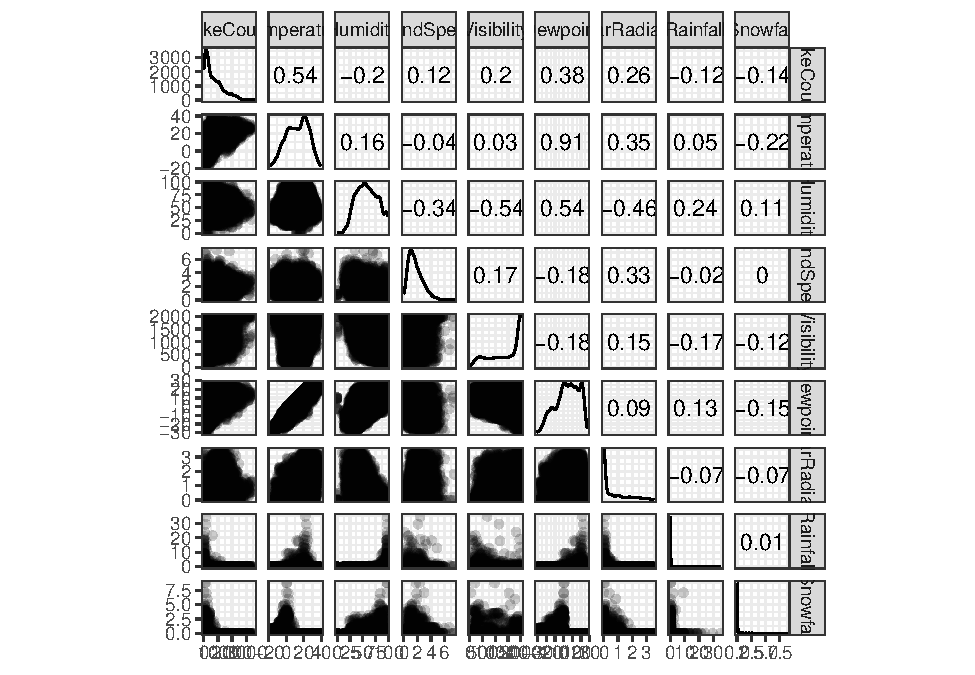
\includegraphics{BikeProject_files/figure-latex/corr-plots-1.pdf}
\includegraphics{BikeProject_files/figure-latex/corr-plots-2.pdf}

Dewpoint and Temperature potentially problematic

\newpage

\hypertarget{bike-demand-by-hour-of-day}{%
\subsection{Bike Demand by Hour of
Day}\label{bike-demand-by-hour-of-day}}

\includegraphics{BikeProject_files/figure-latex/demand-by-day-1.pdf}

\hypertarget{time-series-plots}{%
\subsection{Time Series Plots}\label{time-series-plots}}

\begin{Shaded}
\begin{Highlighting}[]
\FunctionTok{autoplot}\NormalTok{(bikets, }\AttributeTok{.vars =}\NormalTok{ BikeCount) }\SpecialCharTok{+} \FunctionTok{labs}\NormalTok{(}\AttributeTok{title =} \StringTok{"Bike Count by Hour"}\NormalTok{)}
\end{Highlighting}
\end{Shaded}

\includegraphics{BikeProject_files/figure-latex/ts-plots-1.pdf}

\begin{Shaded}
\begin{Highlighting}[]
\FunctionTok{hist}\NormalTok{(bikets}\SpecialCharTok{$}\NormalTok{BikeCount)}
\end{Highlighting}
\end{Shaded}

\includegraphics{BikeProject_files/figure-latex/ts-plots-2.pdf}

\begin{Shaded}
\begin{Highlighting}[]
\NormalTok{bikets\_tall }\SpecialCharTok{\%\textgreater{}\%}
  \FunctionTok{ggplot}\NormalTok{(}\FunctionTok{aes}\NormalTok{(}\AttributeTok{x =}\NormalTok{ Hour, }\AttributeTok{y =}\NormalTok{ Value, }\AttributeTok{color =}\NormalTok{ Measure)) }\SpecialCharTok{+}
  \FunctionTok{geom\_line}\NormalTok{() }\SpecialCharTok{+}
  \FunctionTok{facet\_grid}\NormalTok{(}\AttributeTok{rows =} \FunctionTok{vars}\NormalTok{(Measure), }\AttributeTok{scales =} \StringTok{"free\_y"}\NormalTok{)}
\end{Highlighting}
\end{Shaded}

\includegraphics{BikeProject_files/figure-latex/ts-plots-3.pdf}

\begin{Shaded}
\begin{Highlighting}[]
\FunctionTok{ACF}\NormalTok{(bikets\_tall, Value) }\SpecialCharTok{\%\textgreater{}\%} \FunctionTok{autoplot}\NormalTok{()}
\end{Highlighting}
\end{Shaded}

\includegraphics{BikeProject_files/figure-latex/ts-plots-4.pdf}

\begin{Shaded}
\begin{Highlighting}[]
\FunctionTok{features}\NormalTok{(bikets\_tall, Value, }
         \FunctionTok{c}\NormalTok{(unitroot\_kpss, unitroot\_ndiffs, unitroot\_nsdiffs, ljung\_box))}
\end{Highlighting}
\end{Shaded}

\begin{verbatim}
## Warning: 9 errors (1 unique) encountered for feature 1
## [9] The `urca` package must be installed to use this functionality. It can be installed with install.packages("urca")
\end{verbatim}

\begin{verbatim}
## Warning: 9 errors (1 unique) encountered for feature 2
## [9] The `urca` package must be installed to use this functionality. It can be installed with install.packages("urca")
\end{verbatim}

\begin{verbatim}
## # A tibble: 9 x 4
##   Measure        nsdiffs lb_stat lb_pvalue
##   <chr>            <int>   <dbl>     <dbl>
## 1 BikeCount            1   7152.         0
## 2 Dewpoint             0   8693.         0
## 3 Humidity             1   8128.         0
## 4 Rainfall             0   1243.         0
## 5 Snowfall             0   8384.         0
## 6 SolarRadiation       1   7616.         0
## 7 Temperature          1   8706.         0
## 8 Visibility           0   7599.         0
## 9 WindSpeed            0   5375.         0
\end{verbatim}

KPSS and Ljung-Box Test both indicate (auto)correlation within each
variable.

\hypertarget{pca}{%
\subsection{PCA}\label{pca}}

\begin{Shaded}
\begin{Highlighting}[]
\NormalTok{bike}\SpecialCharTok{$}\NormalTok{Hour }\OtherTok{=} \FunctionTok{as.factor}\NormalTok{(bike}\SpecialCharTok{$}\NormalTok{Hour)}

\CommentTok{\# Correct for skewness for PCA purposes}
\NormalTok{quantData }\OtherTok{=}\NormalTok{ bike }\SpecialCharTok{\%\textgreater{}\%}
  \FunctionTok{select\_if}\NormalTok{(is.numeric)}
\NormalTok{skewnessVec }\OtherTok{=}\NormalTok{ quantData }\SpecialCharTok{\%\textgreater{}\%} \FunctionTok{sapply}\NormalTok{(., e1071}\SpecialCharTok{::}\NormalTok{skewness)}

\NormalTok{skewnessCriterion }\OtherTok{=} \FunctionTok{abs}\NormalTok{(skewnessVec)}\SpecialCharTok{\textgreater{}} \DecValTok{1}

\NormalTok{quantDataSkewedYJ }\OtherTok{=}\NormalTok{ quantData }\SpecialCharTok{\%\textgreater{}\%}
  \FunctionTok{select\_if}\NormalTok{(skewnessCriterion) }\SpecialCharTok{\%\textgreater{}\%}
  \FunctionTok{preProcess}\NormalTok{(}\AttributeTok{method =} \StringTok{\textquotesingle{}YeoJohnson\textquotesingle{}}\NormalTok{) }\SpecialCharTok{\%\textgreater{}\%}
  \FunctionTok{predict}\NormalTok{(quantData }\SpecialCharTok{\%\textgreater{}\%} \FunctionTok{select\_if}\NormalTok{(skewnessCriterion)) }\CommentTok{\# apply Yeo{-}Johnson transformation}

\NormalTok{quantDataNotSkewed }\OtherTok{=}\NormalTok{ quantData }\SpecialCharTok{\%\textgreater{}\%}
  \FunctionTok{select\_if}\NormalTok{(}\SpecialCharTok{!}\NormalTok{skewnessCriterion)}

\NormalTok{quantDataCombined }\OtherTok{=} \FunctionTok{cbind}\NormalTok{(quantDataSkewedYJ, quantDataNotSkewed)}
\CommentTok{\#}

\CommentTok{\# start PCA}
\NormalTok{bikeCountPCA }\OtherTok{=} \FunctionTok{prcomp}\NormalTok{(quantDataCombined,}\AttributeTok{scale=}\ConstantTok{TRUE}\NormalTok{,}\AttributeTok{center=}\ConstantTok{TRUE}\NormalTok{)}
\NormalTok{XtransformPC }\OtherTok{=} \FunctionTok{data.frame}\NormalTok{(bikeCountPCA}\SpecialCharTok{$}\NormalTok{x)}

\FunctionTok{screeplot}\NormalTok{(bikeCountPCA,}\AttributeTok{type=}\StringTok{\textquotesingle{}lines\textquotesingle{}}\NormalTok{) }\CommentTok{\# First two PCs are informative}
\end{Highlighting}
\end{Shaded}

\includegraphics{BikeProject_files/figure-latex/PCA-1.pdf}

\begin{Shaded}
\begin{Highlighting}[]
\FunctionTok{ggplot}\NormalTok{(}\AttributeTok{data =}\NormalTok{ XtransformPC, }\FunctionTok{aes}\NormalTok{(}\AttributeTok{x =}\NormalTok{ PC1, }\AttributeTok{y =}\NormalTok{ PC2)) }\SpecialCharTok{+}
  \FunctionTok{geom\_point}\NormalTok{() }\SpecialCharTok{+}
  \FunctionTok{coord\_cartesian}\NormalTok{(}\AttributeTok{xlim =} \FunctionTok{c}\NormalTok{(}\FunctionTok{min}\NormalTok{(XtransformPC}\SpecialCharTok{$}\NormalTok{PC1,XtransformPC}\SpecialCharTok{$}\NormalTok{PC2),}\FunctionTok{max}\NormalTok{(XtransformPC}\SpecialCharTok{$}\NormalTok{PC1,XtransformPC}\SpecialCharTok{$}\NormalTok{PC2)), }
                  \AttributeTok{ylim =} \FunctionTok{c}\NormalTok{(}\FunctionTok{min}\NormalTok{(XtransformPC}\SpecialCharTok{$}\NormalTok{PC1,XtransformPC}\SpecialCharTok{$}\NormalTok{PC2),}\FunctionTok{max}\NormalTok{(XtransformPC}\SpecialCharTok{$}\NormalTok{PC1,XtransformPC}\SpecialCharTok{$}\NormalTok{PC2)))}\SpecialCharTok{+}
  \FunctionTok{ggtitle}\NormalTok{(}\StringTok{"Summarizing via PCA"}\NormalTok{)}
\end{Highlighting}
\end{Shaded}

\includegraphics{BikeProject_files/figure-latex/PCA-2.pdf}

\begin{Shaded}
\begin{Highlighting}[]
\CommentTok{\# Closer inspection of most extreme observation (bottom right)}
\FunctionTok{filter}\NormalTok{(bike,XtransformPC}\SpecialCharTok{$}\NormalTok{PC1 }\SpecialCharTok{==} \FunctionTok{max}\NormalTok{(XtransformPC}\SpecialCharTok{$}\NormalTok{PC1)) }\CommentTok{\# doesn\textquotesingle{}t look very unusual besides high Humidity}
\end{Highlighting}
\end{Shaded}

\begin{verbatim}
## # A tibble: 1 x 14
##   Date       BikeCount Hour  Temperature Humidity WindSpeed Visibility Dewpoint
##   <chr>          <dbl> <fct>       <dbl>    <dbl>     <dbl>      <dbl>    <dbl>
## 1 16/05/2018       151 13           21.8       97       2.4        682     21.2
## # ... with 6 more variables: SolarRadiation <dbl>, Rainfall <dbl>,
## #   Snowfall <dbl>, Seasons <fct>, Holiday <fct>, FunctionalDay <fct>
\end{verbatim}

\hypertarget{feature-engineering}{%
\subsection{Feature Engineering}\label{feature-engineering}}

\begin{Shaded}
\begin{Highlighting}[]
\CommentTok{\# Extract features from date}
\NormalTok{bike}\SpecialCharTok{$}\NormalTok{Day }\OtherTok{=} \FunctionTok{factor}\NormalTok{(}\FunctionTok{format}\NormalTok{(bikets}\SpecialCharTok{$}\NormalTok{Hour, }\StringTok{"\%d"}\NormalTok{))}
\NormalTok{bike}\SpecialCharTok{$}\NormalTok{Month }\OtherTok{=} \FunctionTok{factor}\NormalTok{(}\FunctionTok{months}\NormalTok{(bikets}\SpecialCharTok{$}\NormalTok{Hour, }\AttributeTok{abbreviate=}\NormalTok{ T)) }
\NormalTok{bike}\SpecialCharTok{$}\NormalTok{WeekDay }\OtherTok{=} \FunctionTok{factor}\NormalTok{(}\FunctionTok{wday}\NormalTok{(bikets}\SpecialCharTok{$}\NormalTok{Hour, }\AttributeTok{label =}\NormalTok{F, }\AttributeTok{week\_start =} \DecValTok{1}\NormalTok{), }\AttributeTok{ordered =}\NormalTok{ F)}

\CommentTok{\# drop last 3 rows since we\textquotesingle{}re not using those. (Similar to Fold 51 in create\_cv\_folds.R)}
\NormalTok{bike }\OtherTok{=} \FunctionTok{slice}\NormalTok{(bike, }\DecValTok{1}\SpecialCharTok{:}\NormalTok{(}\FunctionTok{n}\NormalTok{() }\SpecialCharTok{{-}} \DecValTok{3}\NormalTok{))}

\CommentTok{\# convert categorical features to numeric encoding}
\NormalTok{factors }\OtherTok{=} \FunctionTok{c}\NormalTok{(}\StringTok{"Seasons"}\NormalTok{, }\StringTok{"Holiday"}\NormalTok{, }\StringTok{"FunctionalDay"}\NormalTok{, }\StringTok{"Day"}\NormalTok{, }\StringTok{"Month"}\NormalTok{, }\StringTok{"WeekDay"}\NormalTok{)}
\NormalTok{bike[,factors] }\OtherTok{=} \FunctionTok{sapply}\NormalTok{(bike[,factors], unclass)}
\NormalTok{bike[,factors] }\OtherTok{\textless{}{-}} \FunctionTok{lapply}\NormalTok{(bike[,factors], as.factor)}

\CommentTok{\# create dummy vars}
\NormalTok{XQual }\OtherTok{=}\NormalTok{ bike }\SpecialCharTok{\%\textgreater{}\%} 
  \FunctionTok{select}\NormalTok{(}\SpecialCharTok{{-}}\FunctionTok{c}\NormalTok{(Date,BikeCount)) }\SpecialCharTok{\%\textgreater{}\%}
  \FunctionTok{select\_if}\NormalTok{(is.factor)}
\NormalTok{dummyModel }\OtherTok{=} \FunctionTok{dummyVars}\NormalTok{(}\SpecialCharTok{\textasciitilde{}}\NormalTok{., }\AttributeTok{data =}\NormalTok{ XQual, }\AttributeTok{fullRank=}\ConstantTok{TRUE}\NormalTok{)}
\NormalTok{XQualDummy }\OtherTok{=} \FunctionTok{predict}\NormalTok{(dummyModel, XQual)}
\NormalTok{XQuan }\OtherTok{=}\NormalTok{ bike }\SpecialCharTok{\%\textgreater{}\%} \FunctionTok{select}\NormalTok{(}\SpecialCharTok{{-}}\FunctionTok{c}\NormalTok{(}\FunctionTok{names}\NormalTok{(XQual),Date,BikeCount))}
\NormalTok{XFull }\OtherTok{=} \FunctionTok{cbind}\NormalTok{(XQualDummy, XQuan)}
\end{Highlighting}
\end{Shaded}

\hypertarget{imputation}{%
\subsection{Imputation}\label{imputation}}

\begin{Shaded}
\begin{Highlighting}[]
\CommentTok{\# Imputing values for Humidity using KNN}
\CommentTok{\# BikeCount NA values should be predicted rather than imputed since it is the supervisor and not a feature}
\DocumentationTok{\#\#\#}

\NormalTok{XFull }\OtherTok{=}\NormalTok{ XFull }\SpecialCharTok{\%\textgreater{}\%}
  \FunctionTok{mutate}\NormalTok{(}\AttributeTok{Humidity =} \FunctionTok{ifelse}\NormalTok{(Humidity }\SpecialCharTok{==} \DecValTok{0}\NormalTok{, }\ConstantTok{NA}\NormalTok{, Humidity))}\SpecialCharTok{\%\textgreater{}\%} \CommentTok{\# convert 0 to NA before imputing}
  \FunctionTok{select}\NormalTok{(Humidity) }\SpecialCharTok{\%\textgreater{}\%}
  \FunctionTok{preProcess}\NormalTok{(}\AttributeTok{method=}\StringTok{\textquotesingle{}knnImpute\textquotesingle{}}\NormalTok{) }\SpecialCharTok{\%\textgreater{}\%} \CommentTok{\# Note that this automatically centers and scales Humidity}
  \FunctionTok{predict}\NormalTok{(}\AttributeTok{newdata =}\NormalTok{ XFull)}
\end{Highlighting}
\end{Shaded}

\hypertarget{modeling}{%
\section{Modeling}\label{modeling}}

\hypertarget{time-series}{%
\subsection{Time Series}\label{time-series}}

\begin{itemize}
\tightlist
\item
  Prophet
\item
  fasster
\end{itemize}

\begin{Shaded}
\begin{Highlighting}[]
\FunctionTok{library}\NormalTok{(fable.prophet)}

\NormalTok{holidays }\OtherTok{\textless{}{-}}\NormalTok{ bikets }\SpecialCharTok{\%\textgreater{}\%} 
  \FunctionTok{filter}\NormalTok{(Holiday }\SpecialCharTok{==} \StringTok{"Holiday"}\NormalTok{) }\SpecialCharTok{\%\textgreater{}\%}
  \FunctionTok{mutate}\NormalTok{(}\AttributeTok{ds =} \FunctionTok{as.Date}\NormalTok{(Hour)) }\SpecialCharTok{\%\textgreater{}\%}
  \FunctionTok{distinct}\NormalTok{(ds) }\SpecialCharTok{\%\textgreater{}\%} 
  \FunctionTok{mutate}\NormalTok{(}\AttributeTok{holiday =} \StringTok{"holiday"}\NormalTok{)}

\NormalTok{fit }\OtherTok{\textless{}{-}}\NormalTok{ bikets }\SpecialCharTok{\%\textgreater{}\%}
  \FunctionTok{model}\NormalTok{(}
    \AttributeTok{mdl =} \FunctionTok{prophet}\NormalTok{(BikeCount }\SpecialCharTok{\textasciitilde{}} \FunctionTok{season}\NormalTok{(}\AttributeTok{period =} \StringTok{"day"}\NormalTok{, }\AttributeTok{type =} \StringTok{"multiplicative"}\NormalTok{) }\SpecialCharTok{+} \FunctionTok{season}\NormalTok{(}\AttributeTok{period =} \StringTok{"week"}\NormalTok{, }\AttributeTok{type =} \StringTok{"multiplicative"}\NormalTok{) }\SpecialCharTok{+} \FunctionTok{holiday}\NormalTok{(}\AttributeTok{holidays =}\NormalTok{ holidays)),}
\NormalTok{  )}
\FunctionTok{components}\NormalTok{(fit) }\SpecialCharTok{\%\textgreater{}\%} \FunctionTok{autoplot}\NormalTok{()}
\end{Highlighting}
\end{Shaded}

\hypertarget{machine-learning}{%
\subsection{Machine Learning}\label{machine-learning}}

\hypertarget{xgboost}{%
\subsubsection{XGBoost}\label{xgboost}}

\begin{Shaded}
\begin{Highlighting}[]
\NormalTok{myTuneGrid }\OtherTok{=} \FunctionTok{data.frame}\NormalTok{(}\StringTok{\textquotesingle{}nrounds\textquotesingle{}}\OtherTok{=}\FunctionTok{c}\NormalTok{(}\DecValTok{200}\NormalTok{,}\DecValTok{500}\NormalTok{), }\CommentTok{\#grid still needs tuning}
                       \StringTok{\textquotesingle{}max\_depth\textquotesingle{}}\OtherTok{=} \DecValTok{4}\NormalTok{,}
                       \StringTok{\textquotesingle{}eta\textquotesingle{}} \OtherTok{=} \FloatTok{0.01}\NormalTok{,}
                       \StringTok{\textquotesingle{}gamma\textquotesingle{}} \OtherTok{=} \FunctionTok{c}\NormalTok{(}\DecValTok{0}\NormalTok{,}\FloatTok{0.1}\NormalTok{),}
                       \StringTok{\textquotesingle{}colsample\_bytree\textquotesingle{}} \OtherTok{=} \FloatTok{0.8}\NormalTok{,}
                       \StringTok{\textquotesingle{}min\_child\_weight\textquotesingle{}} \OtherTok{=} \DecValTok{1}\NormalTok{,}
                       \StringTok{\textquotesingle{}subsample\textquotesingle{}} \OtherTok{=} \FloatTok{0.8}\NormalTok{) }

\NormalTok{myTrainControl }\OtherTok{=} \FunctionTok{trainControl}\NormalTok{(}\AttributeTok{method=}\StringTok{"timeslice"}\NormalTok{, }
                              \AttributeTok{initialWindow =} \FunctionTok{nrow}\NormalTok{(bike)}\SpecialCharTok{{-}}\NormalTok{(}\DecValTok{50}\SpecialCharTok{*}\DecValTok{24}\NormalTok{),}
                              \AttributeTok{horizon =} \DecValTok{24}\NormalTok{, }
                              \AttributeTok{skip =} \DecValTok{23}\NormalTok{,}
                              \AttributeTok{fixedWindow =} \ConstantTok{TRUE}\NormalTok{)}


\NormalTok{boostOut }\OtherTok{=} \FunctionTok{train}\NormalTok{(XFull , bike}\SpecialCharTok{$}\NormalTok{BikeCount,}
                 \AttributeTok{method =} \StringTok{"xgbTree"}\NormalTok{,}
                 \AttributeTok{tuneGrid =}\NormalTok{ myTuneGrid,}
                 \AttributeTok{trControl =}\NormalTok{ myTrainControl)}

\NormalTok{boostOut}\SpecialCharTok{$}\NormalTok{bestTune}
\end{Highlighting}
\end{Shaded}

\begin{verbatim}
##   nrounds max_depth  eta gamma colsample_bytree min_child_weight subsample
## 2     500         4 0.01   0.1              0.8                1       0.8
\end{verbatim}

\begin{Shaded}
\begin{Highlighting}[]
\NormalTok{boostOut}\SpecialCharTok{$}\NormalTok{results}
\end{Highlighting}
\end{Shaded}

\begin{verbatim}
##    eta max_depth gamma colsample_bytree min_child_weight subsample nrounds
## 1 0.01         4   0.0              0.8                1       0.8     200
## 2 0.01         4   0.1              0.8                1       0.8     500
##       RMSE  Rsquared      MAE    RMSESD RsquaredSD    MAESD
## 1 407.3302 0.6140617 312.1927 133.75379  0.1595504 96.57607
## 2 292.0835 0.7539397 217.9518  91.47594  0.1240676 65.93860
\end{verbatim}

\begin{Shaded}
\begin{Highlighting}[]
\CommentTok{\#sanity check}
\CommentTok{\#timeSlices \textless{}{-} createTimeSlices(1:nrow(bike), }
\CommentTok{\#                   initialWindow = nrow(bike){-}(50*24), horizon = 24, fixedWindow = T, skip = 23)}

\CommentTok{\#tail(bike[timeSlices$train$Training7581,],1)}
\CommentTok{\#bike[timeSlices$test$Testing7557,]}
\end{Highlighting}
\end{Shaded}

\begin{itemize}
\tightlist
\item
  LSTM
\item
  RNN
\end{itemize}

\end{document}
